% =====================================================================
% Sections to paste into Overleaf (journal version), taken from
% paper/stco/manuscript.tex in the repository evalues4generative.
%
% Each block below REPLACES, in Overleaf, the text that starts with the
% same first line and ends just before the line named in the block header.
% Sections 1-3, 5.1-5.4, 6 and the other appendices are not touched.
%
% Also replace references.bib in Overleaf with paper/stco/references.bib:
% it adds wasserman2020universal (cited in the Discussion),
% mcfadden1974conditional and durkan2020contrastive.
% =====================================================================

% ---------------------------------------------------------------------
% BLOCK 1: Section 4, Betting is predicting
% Replaces from  \section{Betting is predicting}
% up to, not including,  \section{Simulation studies}
% ---------------------------------------------------------------------

\section{Betting is predicting}\label{sec:predictive}
%======================================================================

By Theorem~\ref{thm:growth}, a good score is one whose tilted null is close
to the truth. Choosing such a score is therefore a problem of
sequential prediction: before each real outcome is seen, forecast it as well
as possible from the past. When the null density is known, this problem has a
classical solution, the Bayes factor, and we build on it. We first recall why
the Bayes factor is a product of forecasts and show that the Monte Carlo
e-process has the same structure, with the score in place of the model
(Section~\ref{sec:scores}); we then derive an update rule for the score with a
pathwise guarantee (Section~\ref{sec:simlik}), and its practical version
(Section~\ref{sec:blr}).

For a model $q_\theta$ with prior $\pi_0$, the Bayes factor is the ratio of
the marginal likelihood $m(x_{1:t}) = \int \prod_{i \le t} q_\theta(x_i \mid x_{1:i-1})\,
\pi_0(d\theta)$ to the null density $p_0$. By the chain rule,
\begin{equation}\label{eq:prequential}
\mathrm{BF}_t = \prod_{i=1}^{t} \frac{m_i(x_i)}{p_0(x_i \mid x_{1:i-1})},
\qquad
m_i(x) = \int q_\theta(x \mid x_{1:i-1})\,\pi_{i-1}(d\theta),
\end{equation}
where $\pi_{i-1}$ is the posterior after $i-1$ observations, so $m_i$ is the
posterior predictive of $x_i$. (For a coin with a uniform prior,
$m_i(\text{heads}) = (k+1)/(i+1)$ after $k$ heads in $i-1$ tosses.) Each
factor has conditional mean $\int m_i = 1$ under the null, whatever the prior;
$\log \mathrm{BF}_t$ is the difference between the cumulative log scores of
the learner and of the null \citep{dawid1984present}; and for i.i.d.\ data
and a regular model with $d$ parameters
\[
\log \mathrm{BF}_t = \max_\theta \sum_{i \le t} \log\frac{q_\theta(x_i)}{p_0(x_i)}
- \frac d2 \log t + O_P(1)
\]
\citep{clarke1990information}. The Monte Carlo e-process has the same
structure, and we now look at it from this point of view: the score, through
its tilted null, plays the role of the forecast $m_i$, the simulations that of
the null density $p_0$, and a family of scores $T_\theta$ that of the model
$q_\theta$.

\subsection{Scores are forecasts}\label{sec:scores}

Fix a time $t$ and condition on $\G_t$, so that the action is known. Write
$p_t$ for the density of the simulator's next outcome under that action, and
$q_t$ for the density of the unknown law $Q_t$ of the real next outcome. The
natural score is the density ratio $q_t/p_t$. Neither density can be
evaluated, but their ratio can be estimated by a classifier separating real
outcomes (label 1) from simulator draws (label 0): if the two classes have
prior weights $r$ and $1-r$, Bayes' theorem gives
\[
\Pr(\text{real} \mid x) = \frac{r\, q_t(x)}{r\, q_t(x) + (1-r)\, p_t(x)},
\qquad
\log\frac{\Pr(\text{real} \mid x)}{\Pr(\text{simulated} \mid x)}
= \log\frac{q_t(x)}{p_t(x)} + \log\frac{r}{1-r},
\]
so the classifier's logit is the log ratio up to an additive constant, which
is zero with balanced class weights \citep{thomas2022lfire} and in any case
cancels in \eqref{eq:mc}.

In practice $T_t$ is only an estimate of the true ratio, learned from past
data, and what matters is the density it induces. Reweighting the simulator by
the score as in \eqref{eq:tilt}, which keeps the simulator's outcomes and gives
each a weight proportional to its score, yields the tilted null
\[
\tilde T_t(x) = \frac{T_t(x)\,p_t(x)}{Z_t},
\qquad
Z_t = \E_{P_t}[T_t] = \int T_t(x)\,p_t(x)\,dx ,
\]
a density on the space of outcomes, not the distribution of the score values.
It is the alternative implied by the bet in the sense of
\citet{shafer2021testing}. As $M \to \infty$, $\widehat Z_t \to Z_t$ by the
law of large numbers, so the bet tends to
\[
E_t = \frac{T_t(X_t)}{\widehat Z_t} \;\to\; \frac{T_t(X_t)}{Z_t}
= \frac{\tilde T_t(X_t)}{p_t(X_t)} ,
\]
a likelihood ratio of $\tilde T_t$ against the simulator: a bettor using the
score acts as if the next outcome followed $\tilde T_t$, and wins when real
outcomes fall where $\tilde T_t$ puts more mass than the simulator. If $T_t$
is the true ratio, $Z_t = 1$ and $\tilde T_t = q_t$; otherwise $\tilde T_t$
is the score's forecast of $q_t$. Conversely, any predictive density $f_t$
computed from the past is the tilted null of a score,
\[
T_t = \frac{f_t}{p_t}
\quad\Longrightarrow\quad
Z_t = 1,
\qquad
\tilde T_t = f_t ,
\]
and multiplying a score by a constant $c > 0$ changes neither the bet
\eqref{eq:mc}, where $c$ cancels, nor its tilted null. Scores up to a
constant and predictive densities are therefore the same object. The
correspondence is the familiar one between density ratios and densities,
used for instance in noise-contrastive estimation \citep{gutmann2012noise};
what the Monte Carlo normalisation adds is that the wealth scores these
densities prequentially, without evaluating any of them.

Indeed, by the limit of the bet above, with the betting fraction
$\lambda = 1$ the log wealth tends to
\begin{equation}\label{eq:prequential-wealth}
\log W_t \;=\; \sum_{i \le t} \log E_i \;\to\; \sum_{i \le t} \log \tilde T_i(X_i)
- \sum_{i \le t} \log p_i(X_i),
\end{equation}
which has the form of $\log \mathrm{BF}_t$ in \eqref{eq:prequential}, with
the tilted null $\tilde T_i$ in place of the posterior predictive $m_i$ and
the simulator $p_i$ in place of the null density $p_0$. It is the difference
between the cumulative log scores of two forecasters, each forecast issued
before the outcome it is scored on: the prequential likelihood ratio of
\citet{dawid1984present}. The monitor rejects at level $\alpha$ when the
score's forecasts have predicted the real outcomes $1/\alpha$ times better
than the simulator did. Under the truth, writing
$\log(\tilde T_t/p_t) = \log(q_t/p_t) - \log(q_t/\tilde T_t)$, the expected
increment of \eqref{eq:prequential-wealth} is
\[
\E_{Q_t}\Big[\log\frac{\tilde T_t(X_t)}{p_t(X_t)}\Big]
= \KL(Q_t\|P_t) - \KL(Q_t\|\tilde T_t).
\]
The first term is the information against the simulator and does not depend
on the score; the second is the error of the score's forecast, which by
Gibbs' inequality is nonnegative and vanishes only when $\tilde T_t = Q_t$,
that is, when $T_t$ is the true ratio up to a constant. This is
Theorem~\ref{thm:growth}(ii), and a finite $M$ multiplies the growth by about
$M/(M+1)$ (Theorem~\ref{thm:growth}(iv)). A learned score therefore pays, at
every step, for its error as a forecaster, and only in power.

Reading the score as a forecast scored by the logarithmic loss turns the
choice of the score into a problem of sequential prediction, which
Section~\ref{sec:rules} solves with a Bayesian mixture. The reading also says
where power comes from. A score can only forecast within the family of its
tilted nulls, so the features determine which departures can be detected: for
a score built from the simulator's own parameters, as in SLICE, the tilted
nulls belong to that parametric family, and a departure outside it is
invisible however accurate the score (Section~\ref{sec:exp-concurrent}),
whereas a score learned on features of the outcome reweights the simulator in
directions that need not correspond to any parameter. And since a forecast
need only be issued before the outcome it is scored on, any learner, exact or
approximate, trained online or in advance, keeps the validity of
Theorem~\ref{thm:valid}.

\subsection{From Bayes to the simulation likelihood}\label{sec:rules}\label{sec:exactbayes}\label{sec:simlik}

An update rule for the score must fix the bet on
$X_t$ before $X_t$ is seen, should hedge early on, since an overconfident
forecast can lose all the growth (Theorem~\ref{thm:growth}), and must use
simulations alone, since $p_t$ can only be sampled.

Bayes' rule hedges by averaging over what has not yet been learned. If the
real outcomes followed a model $\{Q_\theta\}$ with prior $\pi_0$, the best
forecast under the model would be its posterior predictive $m_t$, since the
logarithmic score is strictly proper. Section~\ref{sec:scores} supplies a
model: the log-linear scores $s = \theta^\top\phi$ have tilted nulls
$dQ_\theta/dP = \exp\{\theta^\top\phi - \log Z(\theta)\}$, with
$Z(\theta) = \E_P[e^{\theta^\top\phi}]$, an exponential family built on the
simulator. With this model the forecast is an average of tilted nulls,
$m_t = \int q_\theta\,\pi_{t-1}(d\theta)$, its score is
$T_t = \int (dQ_\theta/dP)\,\pi_{t-1}(d\theta)$, and the process becomes a
Bayes factor, the benchmark for what follows.

\begin{proposition}[Predictive scores give the Bayes factor; cf.\ \citealp{clarke1990information}]\label{prop:bayes}
With this score $\E_P[T_t] = 1$, the unlimited-budget factor is
$E_t^\infty = T_t(X_t)$, and
\[
\prod_{i\le t} E_i^\infty = \int \prod_{i \le t} \frac{dQ_\theta}{dP}(X_i)\,\pi_0(d\theta),
\]
the Bayes factor of the tilted family against the simulator. For i.i.d.\ data
and under the usual regularity conditions for Laplace approximations, its
logarithm is $\sup_\theta \sum_{i\le t}\log (dQ_\theta/dP)(X_i) - \frac{d}{2}\log t
+ O_P(1)$, and $t^{-1}$ times it converges to
$\KL(Q\|P) - \inf_\theta \KL(Q\|Q_\theta)$.
\end{proposition}

The proof, in Appendix~\ref{app:proofs}, combines the chain rule with the
Laplace expansion of \citet{clarke1990information}.

Proposition~\ref{prop:bayes} is only a benchmark: Bayes' rule needs the
normalising constant $Z(\theta)$ of every tilt at every step, an integral
against a simulator that can only be sampled.

The Monte Carlo factor provides the way out, because it estimates that
constant from the $M+1$ outcomes. Fix $\theta \in \mathbb{R}^d$ and
$\G_t$-measurable features $\phi_t$, write $U_{t,0} = X_t$ and
$U_{t,k} = Y_{t,k}$, and let
\[
E_t(\theta) = \frac{(M+1)\exp\{\theta^\top\phi_t(U_{t,0})\}}
{\sum_{k=0}^{M}\exp\{\theta^\top\phi_t(U_{t,k})\}}
\]
be the factor \eqref{eq:mc} with score $s_t = \theta^\top\phi_t$. As a
function of $\theta$ it is, up to the constant $M+1$, the probability that the
score assigns to the real outcome among the $M+1$
(Section~\ref{sec:method}), a conditional-logit likelihood whose normalising
constant is a sum over the simulations, always computable. We call
$L_t(\theta) = \prod_{i \le t} E_i(\theta)$ the \emph{simulation likelihood};
its logarithm is the InfoNCE objective of contrastive learning
\citep{oord2018representation,ma2018noise}, which \citet{durkan2020contrastive}
use to estimate likelihood ratios in simulation-based inference. With a prior $\pi_0$ on $\theta$
and posterior $\pi_t \propto \pi_0 L_t$, the \emph{posterior-predictive bet}
is
\[
\bar E_t = \int E_t(\theta)\, \pi_{t-1}(d\theta),
\]
updated by one posterior step per observation instead of a refit on the whole
history. The posterior is a prequential posterior in the sense of
\citet{sinharoy2026prequential}, with loss $-\log E_t(\theta)$ and learning
rate one, the choice that makes the posterior mixture of the bets an
e-process.

\begin{theorem}[Predictive updating on the simulation likelihood]\label{thm:simlik}
Suppose the conditions of Theorem~\ref{thm:valid} hold for each fixed $\theta$
(simulations under the action taken, $\phi_t$ $\G_t$-measurable), that
$\|\phi_t\| \le G$, and that $\pi_0$ is the uniform distribution on a convex
compact set $\Theta \subset \mathbb{R}^d$ with nonempty interior and diameter
at most $2D$.
\begin{enumerate}
  \item[(i)] (Exact factorisation and validity.) The wealth
        $\bar W_t = \prod_{i \le t} \bar E_i$ equals
        $\int L_t(\theta)\,\pi_0(d\theta)$. It is a test martingale under
        $H_0$, for every policy, and it is updated by one posterior step per
        observation, with no recomputation.
  \item[(ii)] (Pathwise regret.) On every sample path, for every
        $t \ge d/(4GD)$,
        \[
        \log \bar W_t \;\ge\; \sup_{\theta \in \Theta} \log L_t(\theta)
        - d \log t - d \log\frac{4eGD}{d}.
        \]
        If the maximiser $\theta^*_t$ of $L_t$ lies in $\Theta$ at distance at
        least $r_t = \sqrt{d/(tG^2)}$ from its boundary, the bound improves to
        $\log \bar W_t \ge \log L_t(\theta_t^*) - \frac d2 \log t
        - \frac d2 \log\frac{e G^2 (2D)^2}{d}$.
  \item[(iii)] (Growth.) Let $g_{M,i}(\theta) = \E[\log E_i(\theta) \mid \G_i]$,
        the conditional growth rate \eqref{eq:growthrate} of the fixed score
        $T = e^{\theta^\top\phi}$, and $g_M(\theta) = g_M(Q, P, e^{\theta^\top\phi})$.
        For every $\theta \in \Theta$, almost surely,
        \[
        \liminf_{t \to \infty} \frac1t \Big(\log \bar W_t - \sum_{i \le t} g_{M,i}(\theta)\Big) \ge 0 .
        \]
        In particular, for i.i.d.\ data under a fixed action and features,
        $\liminf_t t^{-1}\log \bar W_t \ge \sup_{\theta\in\Theta} g_M(\theta)$,
        and, if $\KL(Q\|P) < \infty$, by Theorem~\ref{thm:growth}
        $g_M(\theta) \ge \KL(Q\|P) - \KL(Q\|Q_\theta) - \log\{1 + (\rho_\theta - 1)/(M+1)\}$,
        where $Q_\theta$ is the tilt of $P$ by $\theta^\top\phi$ and
        $\rho_\theta = \E_Q[e^{\theta^\top\phi}]/\E_P[e^{\theta^\top\phi}]$.
\end{enumerate}
\end{theorem}

Part (i) says that the score can be updated by Bayes' rule exactly, even
though the normalising constant $Z(\theta)$ of the tilt is unknown. This is
because the simulation likelihood is not the density of the real outcome under
the tilt, which would need $Z(\theta)$, an integral over all possible
outcomes. It answers the simpler question of Section~\ref{sec:method}: among
the $M+1$ outcomes at hand, which one is the real one? The answer compares the
scores of these $M+1$ outcomes only, so it needs no integral, and its
posterior predictive is the bet itself: updating $\theta$ by Bayes' rule and
betting are the same operation, so the guarantees of Bayesian mixtures hold
for the wealth. It uses less information, and as $M \to \infty$ it recovers
the Bayes factor of Proposition~\ref{prop:bayes}.

Part (ii) holds on every path, with no assumption on the alternative: the
monitor is never more than $d\log t$ behind the best fixed score in the class
chosen in hindsight and evaluated on the same simulations. The argument is the
standard one for Bayesian mixtures of log-concave likelihoods
\citep{kakade2005online,grunwald2007minimum}, applied to the simulation
likelihood, whose log is concave in $\theta$ and whose gradient is bounded by
$2G$. Part (iii) turns this into growth at the rate of the best tilt in the
class, up to the simulation cost of Theorem~\ref{thm:growth}(iii), and
Ville's inequality then gives rejection after about
$\{\log(1/\alpha) + d\log t\}/\sup_\theta g_M(\theta)$ steps.

\subsection{Practical update rules}\label{sec:blr}\label{sec:algorithm}

Exact Bayesian updating needs the posterior $\pi_{t-1}$ at every step. We
replace it by a Gaussian approximation updated in one step per observation,
on either of two losses, or update the forecast directly as martingale
posteriors do. All give valid bets; they differ in where uncertainty comes from
and in the guarantees they carry (Table~\ref{tab:rules}).

The integral in $\bar E_t$ is over $\theta$ only, and any $\G_t$-measurable
distribution $\nu_{t-1}$ on $\theta$, an approximate posterior, in place of
$\pi_{t-1}$ still gives a valid bet
$E^{\nu}_t = \int E_t(\theta)\,\nu_{t-1}(d\theta)$, because $E_t(\theta)$ is
fair for each $\theta$. The price of the approximation is bounded as follows.

\begin{proposition}[Approximate predictive bets]\label{prop:approx}
Let $\nu_{t-1}$ be any $\G_t$-measurable distribution on $\mathbb{R}^d$ with mean
$\bar\theta_{t-1}$ and covariance $\Sigma_{t-1}$, and $\|\phi_t\| \le G$. Then
$E^{\nu}_t$ is an e-value given $\G_t$, and
\[
\log E^{\nu}_t \;\ge\; \E_{\nu_{t-1}}\big[\log E_t(\theta)\big]
\;\ge\; \log E_t(\bar\theta_{t-1}) - \frac{G^2}{2}\,\mathrm{tr}\,\Sigma_{t-1}.
\]
\end{proposition}

\begin{proof}
Validity follows from Fubini's theorem. The first inequality is Jensen's.
The function $\theta \mapsto \log E_t(\theta)$ is concave, with gradient
$\phi_t(U_{t,0}) - \sum_k w_k \phi_t(U_{t,k})$ and Hessian
$-\mathrm{Cov}_w(\phi_t)$, where $w_k \propto e^{\theta^\top\phi_t(U_{t,k})}$;
since $\mathrm{Cov}_w(\phi_t) \preceq \E_w[\phi_t\phi_t^\top] \preceq G^2 I$, with $\E_w$
the average over $k$ of $\phi_t(U_{t,k})$ with weights $w_k$,
Taylor's theorem with integral remainder around $m = \bar\theta_{t-1}$ gives
$\log E_t(\theta) \ge \log E_t(m) + \nabla\log E_t(m)^\top(\theta - m)
- \frac{G^2}{2}\|\theta - m\|^2$ for every $\theta$. Taking the expectation
under $\nu_{t-1}$, the linear term vanishes because $m$ is its mean, and
$\E_{\nu_{t-1}}\|\theta - m\|^2 = \mathrm{tr}\,\Sigma_{t-1}$.
\end{proof}

A predictive bet built from an approximate posterior is therefore never worse
than the plug-in bet at its mean by more than
$\frac{G^2}{2}\sum_i \mathrm{tr}\,\Sigma_{i-1}$. If the posterior precision grows
at least linearly, $\Sigma_i^{-1} \succeq \Sigma_0^{-1} + i\,c_0 I$ for some
$c_0 > 0$, this is at most $\frac{G^2 d}{2c_0}\log t + O(1)$, the order of the
regret in Theorem~\ref{thm:simlik}; such growth needs features that are not
collinear under the simulator and iterates that stay bounded. The Bayesian
learning rule \citep{khan2023bayesian} provides such a posterior. It
approximates a posterior within an exponential family by natural-gradient
descent on the expected loss plus the Kullback--Leibler divergence from the
prior; in a stream, one step per observation with the previous approximation
as the prior \citep{jones2024bong} gives, for a Gaussian
$\nu_t = \mathcal N(\bar\theta_t, S_t^{-1})$ and a per-step loss $\ell_t$,
\begin{equation}\label{eq:blr}
S_t = S_{t-1} + \E_{\nu_{t-1}}[\nabla^2 \ell_t], \qquad
\bar\theta_t = \bar\theta_{t-1} - S_t^{-1}\, \E_{\nu_{t-1}}[\nabla \ell_t],
\end{equation}
which is exact Bayesian updating (the Kalman filter) for a Gaussian likelihood
and one step of online Newton in general. Its cost is $O((M+1)d^2 + d^3)$ per
step with a direct solve, $O((M+1)d^2)$ with rank-one updates of $S_t^{-1}$,
with no refitting and no burn-in.

Two losses are natural. On the simulation likelihood,
$\ell_t(\theta) = -\log E_t(\theta)$, with gradient
$\sum_k w_k \phi_t(U_{t,k}) - \phi_t(U_{t,0})$ and Hessian
$\mathrm{Cov}_w(\phi_t)$; expectations under $\nu_{t-1}$ are computed with
fixed antithetic nodes, and the bet is the average of $E_t(\theta)$ over the
nodes, so Theorem~\ref{thm:simlik} and Proposition~\ref{prop:approx} apply
directly. Alternatively, $\ell_t$ is the balanced logistic loss of classifying
the real outcome (weight one) against the $M$ simulations (weight $1/M$ each),
a generalised posterior \citep{bissiri2016general,sinharoy2026prequential}
that identifies the same tilt through noise-contrastive estimation
\citep{gutmann2012noise}. With the probit approximation
$\E_\nu[\sigma(z^\top\theta)] \approx \sigma(\kappa\bar\eta)$, where
$\bar\eta = z^\top\bar\theta$, $v = z^\top S^{-1}z$ and
$\kappa = (1+\pi v/8)^{-1/2}$, the score is the predictive log-odds
$\kappa\bar\eta$ on the probability scale, inserted in \eqref{eq:mc}; this is
our default. The ratio scale $\bar\eta + v/2$ would be the exact predictive
under an exact posterior, but its premium $v/2$ over-bets where the
approximation is least reliable, and it is the worst score in every experiment
(Supplement, Section~S4). Both losses give scores that start at zero, so the
monitor starts by not betting, and that shrink where the posterior is
uncertain. Features are standardised with simulator draws only, before any
real data are seen, so that the score stays predictable.

The same two classifiers can also be updated without a posterior over their
weights, by updating their predictive directly. In the approach of
\citet{fong2023martingale} one specifies a rule
$m_{t+1} = \mathcal U_t(m_t, X_t)$ and recovers uncertainty by
\emph{predictive resampling}, drawing future outcomes from the current
predictive and updating; this converges when imputing one more outcome does
not move the forecast on average, $\E_{X \sim m_t}[\mathcal U_t(m_t, X)] = m_t$,
the conditionally identically distributed sequences of \citet{berti2004limit}.
Here the learner carries the predictive itself, $\sigma(z^\top\theta_t)$ for
the logistic loss or the softmax $e^{\theta_t^\top z_k}/\sum_{k'} e^{\theta_t^\top z_{k'}}$
over the $M+1$ outcomes for the simulation likelihood, and updates it by
Fisher scoring on the predictive's own log-likelihood,
\begin{equation}\label{eq:mp}
I_t = I_{t-1} + J_t(\theta_{t-1}), \qquad
\theta_t = \theta_{t-1} - I_t^{-1}\, \nabla_t(\theta_{t-1}),
\end{equation}
where $\nabla_t$ is the gradient of the new batch's loss, $J_t$ its Fisher
information, which for both losses does not depend on the labels, and $I_0$ a
prior precision. Under the predictive the gradient has mean zero, so
$\theta_t$ is a martingale, and the bet averages the factor over $N$
predictive-resampling paths, obtained by running \eqref{eq:mp} forward from
$(\theta_{t-1}, I_{t-1})$ on past batches whose labels are drawn from the
predictive ($N = 16$, truncated at $\min(t, 200)$ steps, refreshed every ten
steps). Any learner can be made a martingale-posterior learner in this way:
with the empirical predictive, predictive resampling is the Bayesian
bootstrap, and a random forest fitted with Dirichlet weights on the past steps
is valid as well (Supplement, Section~S4).

\sbox{\widetab}{\begin{tabular}{lll}
\toprule
rule & uncertainty from & guarantee beyond validity \\
\midrule
Bayes on the simulation likelihood & exact posterior & pathwise regret (Theorem~\ref{thm:simlik}) \\
BLR on the simulation likelihood & Gaussian approximation & Theorem~\ref{thm:simlik} up to Proposition~\ref{prop:approx} \\
BLR on the logistic loss (default) & Gaussian approximation & none \\
predictive-first \eqref{eq:mp} & predictive resampling & none \\
\bottomrule
\end{tabular}}%
\begin{table}[t]
\centering
\caption{Update rules for the score (Sections~\ref{sec:simlik}
and~\ref{sec:blr}). All give exactly valid bets; they differ in the source of
uncertainty about the score and in the guarantee they carry beyond validity.
Further variants are in the Supplement.}
\label{tab:rules}
\small
\begin{tabular}{@{}c@{}}\resizebox{\textwidth}{!}{\usebox{\widetab}}\end{tabular}
\end{table}

Algorithm~1 puts the default rule together, the logistic Bayesian learning
rule with the probability-scale predictive; its steps are numbered as in
Figure~\ref{fig:workflow}, and each is followed by the role it plays.

\begin{figure}[t]
\centering
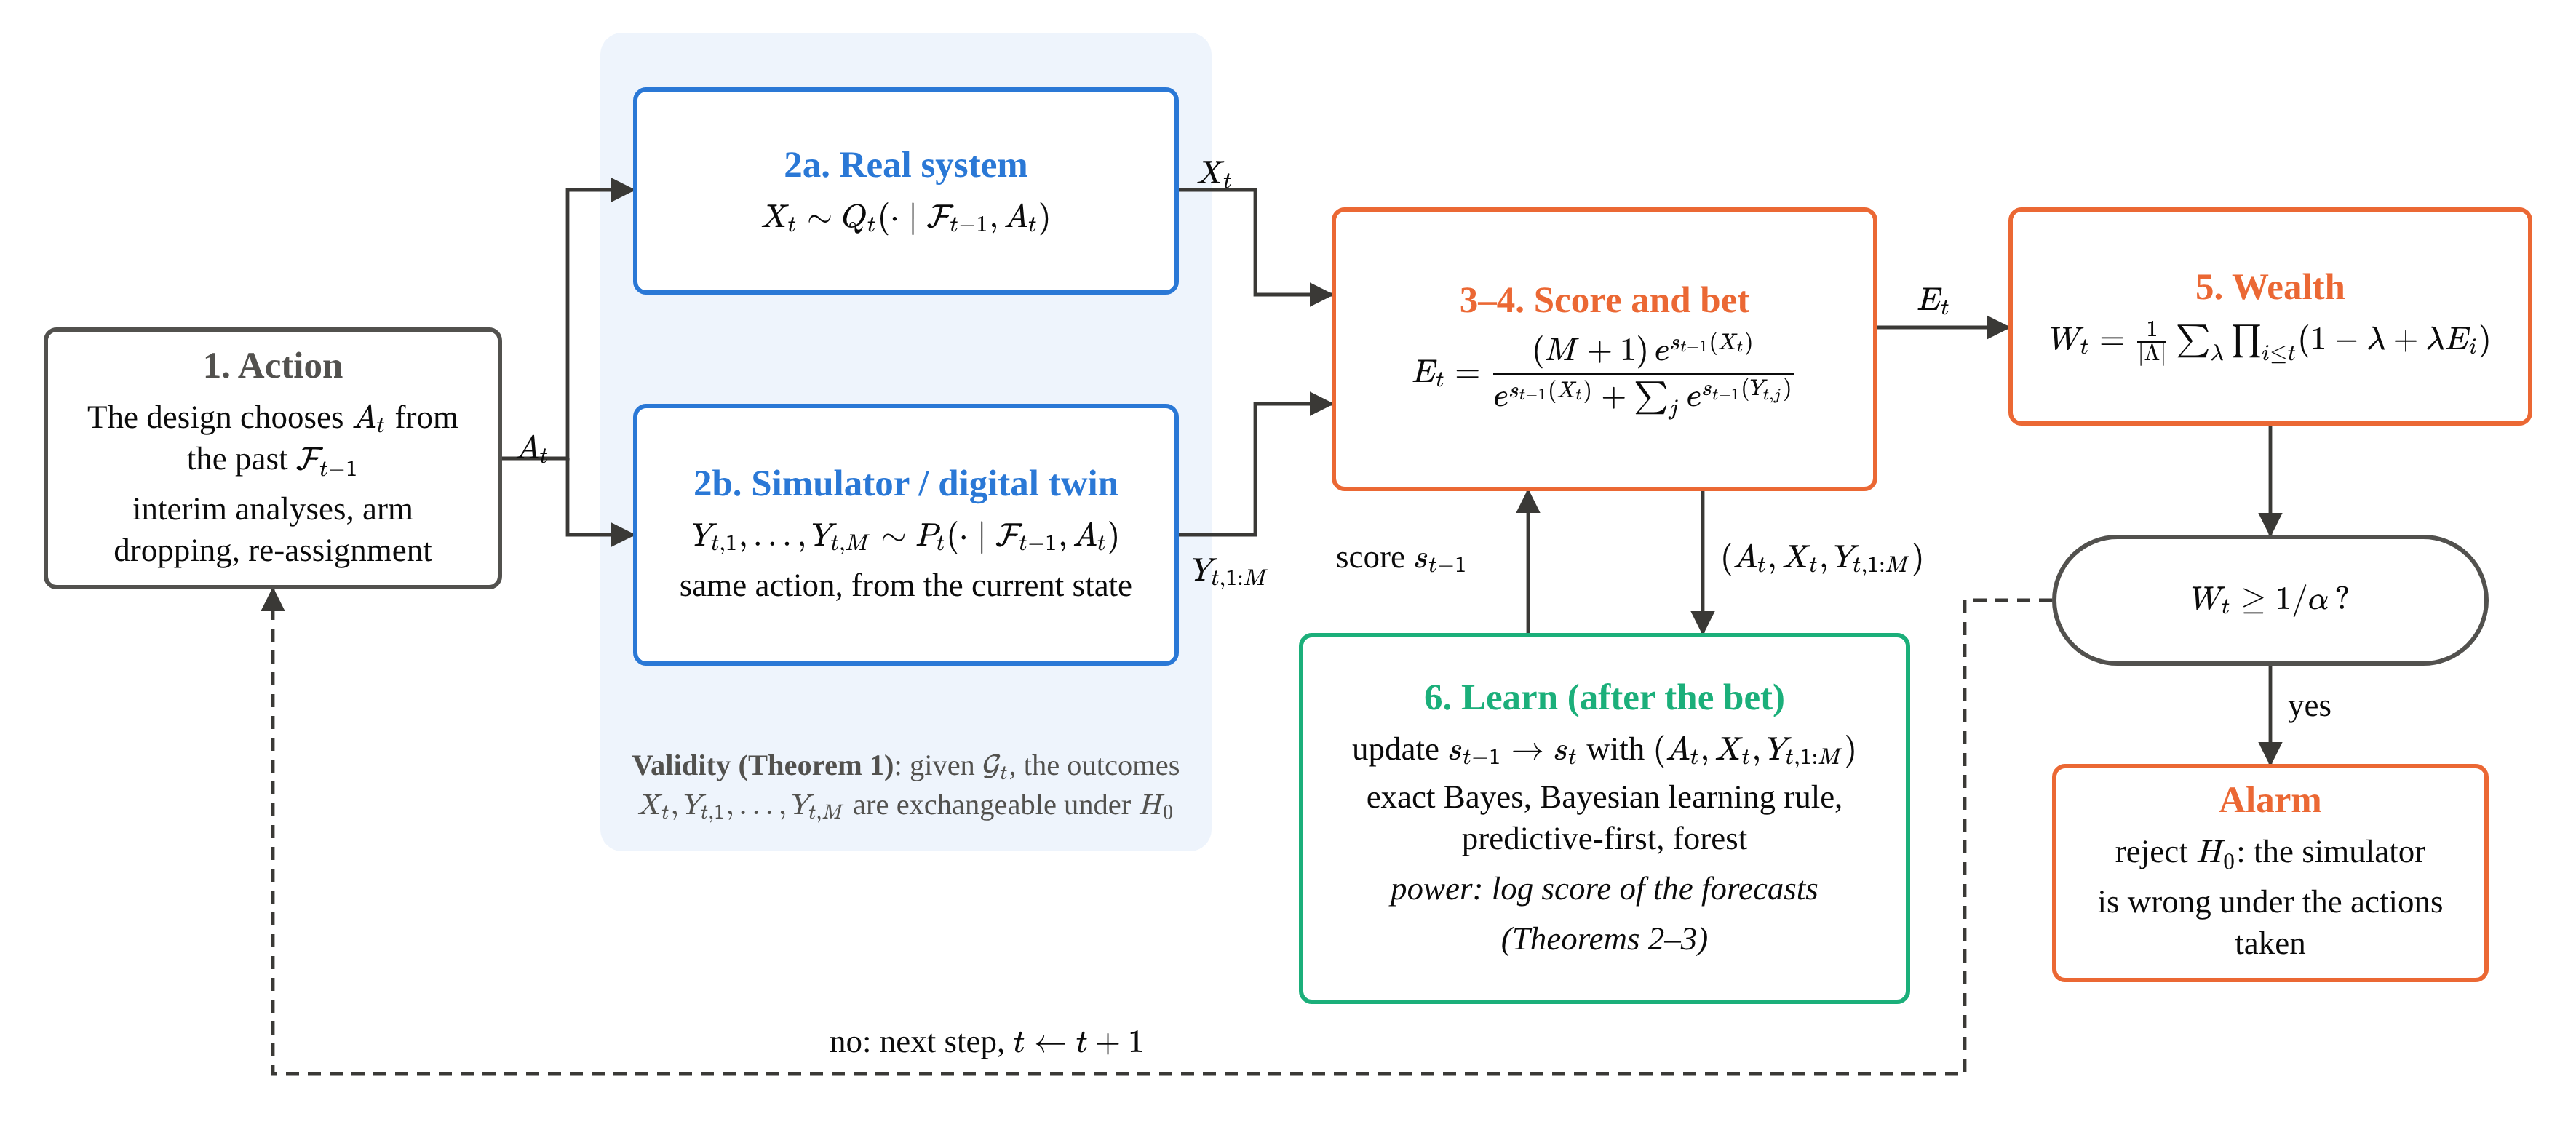
\includegraphics[width=\textwidth]{workflow.png}
\caption{One step of the procedure. The design chooses the action from the
past (1); the real system and the simulator are run under that action and
from the current state (2a, 2b); the current score, fixed before $X_t$ is
seen, turns the $M+1$ outcomes into the bet $E_t$ (3--4), which updates the
wealth (5); the null is rejected when the wealth reaches $1/\alpha$, and
otherwise the learner updates the score with the new outcomes (6) and the
next step begins. Validity rests on the shaded block alone; the learner
affects only power. Algorithm~1 gives the
formulas of each step.}
\label{fig:workflow}
\end{figure}

\paragraph{Algorithm 1 (Monte Carlo e-process with a predictive score).}
\textbf{Input:} a simulator that can be run under any action from any state; a
feature map $z(x)$; the number of simulations $M$; the level $\alpha$; the grid
$\Lambda$ of betting fractions. \textbf{Initialise:} standardise $z$ with
simulator draws only; set $\bar\theta_0 = 0$, $S_0 = I$ (vaguer on the intercept), and
$W_0 = 1$. \textbf{Notation:} $U_{t,0} = X_t$, $U_{t,j} = Y_{t,j}$,
$z_k = z(U_{t,k})$; $s_{t-1}$ is the score fixed at the end of step $t-1$, the
$s_t$ of \eqref{eq:mc}.
\begin{enumerate}
  \item \textbf{Action.} Observe the action $A_t$ chosen by the design from the
        past (arm, prompt, dose). --- It defines the null law $P_t$.
  \item \textbf{Simulate.} Draw $Y_{t,1}, \ldots, Y_{t,M}$ from the simulator
        under $A_t$ from the current state, and observe $X_t$.
        --- Exchangeable with $X_t$ under $H_0$.
  \item \textbf{Score.} For each of the $M+1$ outcomes $x$, compute
        \[
        \begin{gathered}
        \bar\eta = z(x)^\top \bar\theta_{t-1}, \qquad v = z(x)^\top S_{t-1}^{-1} z(x), \\
        \kappa = (1 + \pi v/8)^{-1/2}, \qquad
        s_{t-1}(x) = \mathrm{clip}(\kappa\,\bar\eta,\, -B,\, B) .
        \end{gathered}
        \]
        --- $s_{t-1}$ is the predictive log-odds of ``real'' against
        ``simulated'', an estimate of $\log(q/p)$ shrunk where the posterior is
        uncertain; it forecasts $\tilde T_t \propto p_t\, e^{s_{t-1}}$
        \eqref{eq:tilt}. Clipping at $B$ (we use $B = 30$) keeps the score
        predictable, so validity is unaffected, and makes
        Corollary~\ref{cor:cumulative}(ii) apply.
  \item \textbf{Bet.}
        \[
        E_t = \frac{(M+1)\, e^{s_{t-1}(X_t)}}{e^{s_{t-1}(X_t)} + \sum_{j=1}^{M} e^{s_{t-1}(Y_{t,j})}} .
        \]
        --- Exactly fair under $H_0$ (Theorem~\ref{thm:valid}); close to
        $\tilde T_t(X_t)/p_t(X_t)$ for large $M$.
  \item \textbf{Wealth.} $W_t = |\Lambda|^{-1}\sum_{\lambda\in\Lambda}
        \prod_{i\le t}(1-\lambda+\lambda E_i)$; reject $H_0$ when
        $W_t \ge 1/\alpha$. --- A test martingale; its log is the
        prequential likelihood ratio \eqref{eq:prequential-wealth} of the
        forecasts against the simulator, and it grows at about
        $\frac{M}{M+1}\{\KL(Q\|P) - \KL(Q\|\tilde T)\}$ per step
        (Theorem~\ref{thm:growth}).
  \item \textbf{Learn.} Only now, with labels $y_0 = 1$ for $X_t$ and $y_j = 0$
        for $Y_{t,j}$, weights $w_0 = 1$ and $w_j = 1/M$, and
        $p_k = \sigma(s_{t-1}(U_{t,k}))$, update
        \[
        \begin{gathered}
        \nabla_t = \sum_{k=0}^{M} w_k (p_k - y_k)\, z_k, \qquad
        J_t = \sum_{k=0}^{M} w_k \kappa_k\, p_k (1 - p_k)\, z_k z_k^\top, \\
        S_t = S_{t-1} + J_t, \qquad \bar\theta_t = \bar\theta_{t-1} - S_t^{-1} \nabla_t .
        \end{gathered}
        \]
        --- One step of the Bayesian learning rule \eqref{eq:blr}, with $\kappa_k$
        as in step 3 for $z_k$: $\kappa_k p_k(1-p_k)$ is the derivative of the
        probit approximation $\sigma(\kappa_k\bar\eta_k)$ with respect to
        $\bar\eta_k$, which approximates $\E_\nu[\sigma'(z_k^\top\theta)]$; the score
        stays predictable.
\end{enumerate}
\textbf{Variants.} With the simulation likelihood, steps 3--4 are replaced by
the posterior-predictive mixture $\bar E_t = N^{-1}\sum_b E_t(\theta_b)$ over
posterior nodes $\theta_b$, and step 6 by \eqref{eq:blr} with
$\ell_t = -\log E_t(\theta)$; Theorem~\ref{thm:simlik} and
Proposition~\ref{prop:approx} then apply. With the predictive-first rule,
steps 3 and 6 are replaced by \eqref{eq:mp} and step 4 by the average of the
factor over predictive-resampling paths. In a multi-arm design, one copy of the
algorithm per arm, betting only on that arm's observations, is combined by e-BH
at the end (Section~\ref{sec:trial}).


% ---------------------------------------------------------------------
% BLOCK 2: Sections 5.5 and 5.6, comparison and language-model audit (with Tables 6 and 7)
% Replaces from  \subsection{Comparison with concurrent methods}
% up to, not including,  \section{A multi-arm multi-stage trial designed in silico}
% ---------------------------------------------------------------------

\subsection{Comparison with concurrent methods}\label{sec:exp-concurrent}

The concurrent methods use the same bet and differ in how the score is
chosen, so we run them with the same simulations, mixture over $\lambda$ and
data. For \citet{forre2026anytime} we use the score refitted every ten steps by
maximising the penalised empirical growth, and a score fitted in advance on
simulations from a guessed alternative. For \citet{cortinovis2026slice} we use
SLICE with a single null: an amortised neural ratio network trained on
$2 \times 10^5$ simulations from the simulator's parametrised family
(curvature $b$ for the drift, a location shift per arm for the bandit),
evaluated at a predictable estimate of the parameter. In the bandit both are
run on simulations under the chosen arm, and once as published, with the twin
on random arms. Each task also has an alternative outside SLICE's family: in
the drift the first coordinate is 20\% wider, in the bandit the most pulled
arm keeps its mean and has 50\% larger noise.

\sbox{\widetab}{\begin{tabular}{lrrrrrr}
\toprule
 & \multicolumn{2}{c}{drift} & \multicolumn{2}{c}{bandit} & false & time \\
score & in family & out of family & in family & out of family & alarms & (s) \\
\midrule
ours, BLR logistic & 0.99 (214.5) & 0.73 (321.5) & 1.00 (38) & 1.00 (112) & 2.0--2.2\% & 0.3 / 0.2 \\
ours, simulation likelihood & 0.96 (228.5) & 0.87 (228) & 1.00 (55) & 0.99 (157) & 1.0--1.8\% & 0.3 / 0.15 \\
F\&B, refitted on the past & 0.99 (210) & 0.91 (228) & 1.00 (61) & 0.99 (167) & 1.5--1.8\% & 1.0 / 0.65 \\
F\&B, fitted in advance & 1.00 (57.5) & 0.01 & -- & -- & 4.8\% & -- \\
SLICE, neural ratio, $G = 1$ & 1.00 (66.5) & 0.01 & 1.00 (35) & 0.56 (258) & 1.5--3.3\% & 0.45 / 0.4 \\
F\&B, twin on random arms & -- & -- & \multicolumn{2}{c}{false alarms 100\%} & -- & -- \\
\bottomrule
\end{tabular}}%
\begin{table}[t]
\centering
\caption{Comparison with \citet{forre2026anytime} (F\&B) and
\citet{cortinovis2026slice} (SLICE). Entries: power and, in brackets, median
stopping time; ``in family'': the alternatives of
Sections~\ref{sec:exp-drift} and~\ref{sec:exp-bandit}; ``out of family'':
departures that SLICE's family does not contain. False alarms: range over the
two tasks. Time: computing time per replication on one core, drift / bandit,
excluding the training of SLICE's network. All variants are in the
Supplement.}
\label{tab:concurrent}
\small
\begin{tabular}{@{}c@{}}\resizebox{\textwidth}{!}{\usebox{\widetab}}\end{tabular}
\end{table}

In Table~\ref{tab:concurrent}, conditioning on the action is necessary for
every score: run as published, the refitted score of
\citet{forre2026anytime} rejects the true null in every bandit run. Scores
that know where the departure lies are fastest inside the family, SLICE after
67 steps on the drift and a score fitted on the true alternative after 58,
against about 210 for scores learned from the data; but outside the family
their power falls to 0.01 on the drift (Remark~\ref{rem:family}), while every
score learned from real against simulated outcomes keeps it. Among the learned
scores, the refit of \citet{forre2026anytime} is slightly more powerful on the
drift task, markedly so against our logistic learner outside the family (0.91
against 0.73), and ours are faster on the bandit (38 against 61 steps inside
the family, 112 against 167 outside). The gap outside the family comes from
the logistic learner, not from the method. On the simulation likelihood, the
objective that the refit maximises, our update has the same median stopping
time as the refit (228 steps), plausibly because the logistic learner's probit
shrinkage keeps its bets small for longer when the signal is weak. Ours cost a
third as much and carry the pathwise guarantee of Theorem~\ref{thm:simlik}.
They average over the uncertainty about the score's parameter, whereas a sequence of refits at a maximiser is in general not the
predictive sequence of any exchangeable model
\citep{fortini2000exchangeability,fortini2024exchangeability}.

\begin{remark}[Inside and outside the family]\label{rem:family}
SLICE bets with $s_t = \log (p_{\hat\theta_{t-1}}/p_{\theta_0})$ within a
parametrised family $\{P_\theta\}$ with null $\theta_0$, so its tilted null is
$P_{\hat\theta_{t-1}}$. Outside the family, $\hat\theta_t$ converges to the
projection $\theta^* = \arg\min_\theta \KL(Q\|P_\theta)$ and the growth tends to
$\KL(Q\|P_{\theta_0}) - \KL(Q\|P_{\theta^*})$ (Theorem~\ref{thm:growth}(ii)).
When $\theta^* = \theta_0$ the score tends to zero and the wealth stops
growing, however large the departure and however good the network. Both
out-of-family alternatives are of this kind: in the drift no curvature $b$
produces a wider first coordinate and the projection is the null itself, and
in the bandit a location shift cannot produce a larger noise. Our features
contain $x_1^2$ and the squared outcome of each arm, so a change of scale moves
the tilted null towards $Q$. Details, and the choice between the NRE-A and
NRE-C estimators \citep{miller2022contrastive}, are in the Supplement.
\end{remark}

\subsection{Auditing a language-model API with adaptively chosen prompts}\label{sec:exp-llm}

Many language models are used through an API, a service that returns the
model's reply to a text, the prompt, without showing which model produced it.
A provider may advertise a model $P$ and answer some queries with a cheaper
substitute, such as $P$ at lower numerical precision or a smaller model. An
audit checks this from the outside, comparing the API's replies with replies
of $P$ to the same prompts, run locally. The API is the real system, the local
copy of $P$ is the simulator and the prompt is the action; neither gives
probabilities, only replies.

As in the routing audit of \citet{cortinovis2026slice}, the prompts ask for
random output (eight random digits, an integer between 1 and 100, a colour,
six coin flips), so that a substitute shows up as a change in the frequencies
of the replies rather than as a wrong answer. The advertised model is
Qwen2.5-1.5B-Instruct \citep{qwen2024qwen25} stored with 8 bits per weight;
the substitutes are the same model with 4 and 3 bits and the smaller
Qwen2.5-0.5B-Instruct. All replies are real outputs of \texttt{llama.cpp}
\citep{gerganov2023llamacpp} at temperature one; only the routing, the choice
of the queries that go to the substitute, is simulated. Either 30\% of all
queries go to the substitute, or 50\% of the colour and number queries and
none of the others. In a last scenario the API answers every query with a
sharpened $P$, which gives $P$'s frequent replies more often, as a lower
temperature would: the most frequent colour goes from 23\% to 44\% of the
replies.

At each step the auditor chooses a prompt, sends it to the API and generates
$M = 8$ replies of $P$ to the same prompt. The prompt is chosen adaptively,
from the bets won so far. For each prompt the auditor computes the average log
growth of its past bets, adds a bonus that shrinks as the prompt is asked more
often, and asks the prompt with the largest sum, so that it tries prompts it
knows little about as well as those that have paid; this is the upper
confidence bound (UCB) rule of bandit problems \citep{lattimore2020bandit},
used here without tuning. No prompt is asked in fewer than a tenth of the
queries: whenever one falls below that share, it is asked next, so that the
score keeps learning on every prompt.

We compare five scores. Two are ours, both on hashed character $n$-grams
with one block of weights per prompt: the logistic BLR of
Section~\ref{sec:blr}, our default, and the simulation-likelihood rule of the
same section, the one covered by Theorem~\ref{thm:simlik}. They reweight the
replies of $P$ prompt by prompt and need no reply of the substitute. The score
of \citet{forre2026anytime} is used in its two versions: refitted every ten
steps on the whole history by maximising the empirical growth, on the same
features, and fitted in advance to separate a guessed substitute $R$ from
$P$. SLICE assumes that $R$ answers a fraction $\theta$ of the queries, the
same for all prompts, and estimates $\theta$. The score fitted in advance and
SLICE learn $R$ before the audit from 500 replies per prompt of the 4-bit
model, so they guess wrong for the 3-bit and 0.5B substitutes; routing that
depends on the prompt lies outside SLICE's family, and the sharpened $P$ lies
outside it in a stronger sense, since it is closer to $P$ than to $R$.

\sbox{\widetab}{\begin{tabular}{llrrrrrl}
\toprule
 & & \multicolumn{4}{c}{substitute} & false & growth \\
\cmidrule(lr){3-6}
score & routing & 4-bit & 3-bit & 0.5B & sharpened $P$ & alarms & guarantee \\
\midrule
\multicolumn{8}{l}{\emph{prompts drawn uniformly (as published)}} \\
SLICE & all & 82 & 149 (0.96) & 110 (0.99) & never & 0.0\% & -- \\
 & two & 76 &  & 107 &  & & \\
\addlinespace[3pt]
F\&B, fitted in advance & all & 44 & 72 & 70 & never & 3.5\% & -- \\
 & two & 39 &  & 59 &  & & \\
\addlinespace[3pt]
F\&B, refitted & all & 251 (0.83) & 170 (0.98) & 102 & 93 & 3.8\% & -- \\
 & two & 200 (0.93) &  & 75 &  & & \\
\addlinespace[3pt]
ours, logistic BLR & all & 255 (0.72) & 209 (0.96) & 123 & 86 & 5.3\% & -- \\
 & two & 219 (0.83) &  & 77 &  & & \\
\addlinespace[3pt]
ours, simulation likelihood & all & 254 (0.69) & 195 (0.99) & 100 & 151 & 4.3\% & Thm~\ref{thm:simlik}$^*$ \\
 & two & 219 (0.85) &  & 62 &  & & \\
\midrule
\multicolumn{8}{l}{\emph{prompts chosen by UCB (our design)}} \\
SLICE & all & 72 & 109 (0.97) & 95 & never & 0.0\% & -- \\
 & two & 57 &  & 57 &  & & \\
\addlinespace[3pt]
F\&B, fitted in advance & all & \textbf{41} & \textbf{50} & \textbf{48} & never & 2.5\% & -- \\
 & two & \textbf{30} &  & \textbf{23} &  & & \\
\addlinespace[3pt]
F\&B, refitted & all & 177 (0.98) & 131 (0.98) & 94 & \textbf{78} & 3.3\% & -- \\
 & two & 107 &  & 51 &  & & \\
\addlinespace[3pt]
average$^\ddagger$ & all & 50 & 66 & 56 & 95 & 2.8\% & -- \\
 & two & 39 &  & 29 &  & & \\
\addlinespace[3pt]
ours, logistic BLR & all & 218 (0.96) & 162 (0.99) & 109 & \textbf{78} & 3.0\% & -- \\
 & two & 136 &  & 52 &  & & \\
\addlinespace[3pt]
ours, simulation likelihood & all & 193 (0.92) & 138 (0.99) & 83 & 130 & 1.5\% & Thm~\ref{thm:simlik}$^*$ \\
 & two & 119 (0.99) &  & 36 &  & & \\
\bottomrule
\end{tabular}}%
\begin{table}[t]
\centering
\caption{Auditing a language-model API (Section~\ref{sec:exp-llm}): median
number of queries to an alarm (fewest in bold), rounded to an integer, over
the runs that reject within 400 queries, with the power when below one;
``never'': no run rejects. Routing: ``all'', the substitute answers 30\% of
all queries (the sharpened $P$ answers every query); ``two'', it answers 50\%
of the colour and number queries only. SLICE and the score fitted in advance
are given replies of the 4-bit substitute; the refitted score and ours are
given none. False alarms: rejections of the true null within 400 queries
(Monte Carlo standard error about 1.1\%); a twin that answers a random prompt
raises a false alarm in every run. $^\ddagger$Average of the wealths of ours
(logistic) and of the score fitted in advance. $^*$For the exact posterior;
the one-step Gaussian update used here is covered by
Proposition~\ref{prop:approx}.}
\label{tab:llm}
\small
\setlength{\tabcolsep}{4pt}
\begin{tabular}{@{}c@{}}\resizebox{\textwidth}{!}{\usebox{\widetab}}\end{tabular}
\end{table}

\sbox{\widetab}{\begin{tabular}{llrrrrrrrrr}
\toprule
 & & \multicolumn{2}{c}{4-bit} & 3-bit & \multicolumn{2}{c}{0.5B} & sharpened & prepared & \multicolumn{2}{c}{ms per query} \\
\cmidrule(lr){3-4}\cmidrule(lr){5-5}\cmidrule(lr){6-7}\cmidrule(lr){8-8}\cmidrule(lr){10-11}
score & to the alarm & all & two & all & all & two & $P$, all & ($10^3$) & 400 & 1600 \\
\midrule
SLICE & replies ($10^3$) & 6.6 & 6.5 & 6.9 & 6.8 & 6.5 & never & 6.0 & 1.6 & 2.3 \\
 & computing (s) & 0.12 & 0.09 & 0.17 & 0.15 & 0.09 & never & & & \\
\addlinespace[3pt]
F\&B, fitted in advance & replies ($10^3$) & 6.3 & 6.2 & 6.4 & 6.4 & 6.2 & never & 6.0 & 1.0 & 1.2 \\
 & computing (s) & \textbf{0.05} & \textbf{0.06} & \textbf{0.07} & \textbf{0.06} & \textbf{0.03} & never & & & \\
\addlinespace[3pt]
F\&B, refitted & replies ($10^3$) & \textbf{2.2} & \textbf{1.7} & \textbf{1.8} & 1.5 & 1.2 & \textbf{1.4} & 0.8 & 8.0 & 53.4 \\
 & computing (s) & 0.60 & 0.29 & 0.34 & 0.17 & 0.07 & 0.12 & & & \\
\addlinespace[3pt]
average$^\ddagger$ & replies ($10^3$) & 7.2 & 7.1 & 7.3 & 7.2 & 7.0 & 7.6 & 6.8 & 2.5 & 2.7 \\
 & computing (s) & 0.15 & 0.12 & 0.20 & 0.17 & 0.08 & 0.27 & & & \\
\addlinespace[3pt]
ours, logistic BLR & replies ($10^3$) & 2.5 & 1.9 & 2.1 & 1.7 & 1.2 & \textbf{1.4} & 0.8 & 1.4 & 1.3 \\
 & computing (s) & 0.33 & 0.21 & 0.24 & 0.15 & 0.08 & \textbf{0.11} & & & \\
\addlinespace[3pt]
ours, simulation likelihood & replies ($10^3$) & 2.3 & 1.8 & 1.9 & \textbf{1.5} & \textbf{1.1} & 1.8 & 0.8 & 2.1 & 2.2 \\
 & computing (s) & 0.48 & 0.30 & 0.33 & 0.19 & 0.08 & 0.30 & & & \\
\bottomrule
\end{tabular}}%
\begin{table}[t]
\centering
\caption{Cost of reaching the alarm in the audit of
Section~\ref{sec:exp-llm}, with the prompts chosen by UCB: medians over the
runs of Table~\ref{tab:llm} that reject (lowest in bold). Replies: replies
generated by language models, those prepared before the audit (thousands,
column 9) plus $M = 8$ per query. Computing: time spent on the bets and the
updates up to the alarm, on one core. Milliseconds per query: computing time
over 400 and 1600 queries under the null; it grows with the history for the
refit, which revisits the whole history at every refit, and more slowly for
SLICE, which re-estimates its routing fraction from all past replies.
Generating the replies takes 2 to 8 seconds per query on four CPU cores.
$^\ddagger$As in Table~\ref{tab:llm}.}
\label{tab:llmcost}
\small
\setlength{\tabcolsep}{4pt}
\begin{tabular}{@{}c@{}}\resizebox{\textwidth}{!}{\usebox{\widetab}}\end{tabular}
\end{table}

Choosing the prompts helps every score (Table~\ref{tab:llm}): with our
adaptive design every score needs fewer queries than with uniformly drawn
prompts, in every scenario in which it rejects and up to 61\% fewer, and our
scores gain up to 0.24 in power; the auditor learns to ask for a colour more
often, because that is where the substitutes differ most. Validity requires
the conditioning: comparing the API's reply with replies of $P$ to a random
prompt, rather than to the same prompt, raises a false alarm in every run,
whereas the conditioned monitors raise false alarms in at most 5.3\% of the
runs, within Monte Carlo error of the nominal 5\%.

Knowing the substitute pays when the guess is right and fails when it is not.
With our design the score fitted in advance is the fastest in the five
routing scenarios, after 23 to 50 queries against 36 to 218 for the scores
learned during the audit. When the API sharpens $P$, however, a score fitted
to $R$ has a tilted null close to $R$, hence a growth rate close to
$\KL(Q\|P) - \KL(Q\|R) < 0$ by Theorem~\ref{thm:growth}: it never rejects,
nor does SLICE, which estimates a routing fraction of zero and stops betting.
The three scores learned during the audit reject in every run, after 78 to
130 queries. The average of the wealths of the logistic score and of the
score fitted in advance keeps the best of both: it is within 16 queries of
the faster component in the routing scenarios, and rejects after 95 queries
when the guess is wrong.

Our simulation-likelihood rule and the refit of \citet{forre2026anytime} both
learn the score during the audit and need no guess about the substitute. With
our design the refit needs 5 to 10\% fewer queries on the 4-bit and 3-bit
substitutes and 40\% fewer on the sharpened $P$ (78 against 130), whereas our
rule needs 12 and 29\% fewer on the 0.5B substitute (83 against 94, and 36
against 51); our logistic rule ties with the refit on the sharpened $P$. In
exchange our rule carries the guarantee of Theorem~\ref{thm:simlik}, through
Proposition~\ref{prop:approx} for the one-step update, and its computing time
per query does not grow with the history (Table~\ref{tab:llmcost}): 2.1 and
2.2~ms over 400 and 1600 queries, against 8.0 and 53~ms for the refit, which
revisits the whole history at every refit.

Almost all the running time of the audit goes into the simulator: generating
the $M = 8$ replies of $P$ takes 2 to 8 seconds per query on four CPU cores,
whereas the bet and the update take at most 8~ms over 400 queries, less than
0.5\% of the running time. In these short audits the computing time to the
alarm is therefore at most 0.6~s for every score, and the cost of an alarm is
counted in generated replies, those prepared before the audit plus eight per
query. SLICE and the score fitted in advance prepare 6000 replies, more than
a whole audit, and reach the alarm after 6200 to 6900 replies; the learned
scores prepare 800 replies of $P$, only to standardise the features, and
reach it after 1100 to 2500 (Table~\ref{tab:llmcost}). If one preparation
serves several audits, its cost is shared among them; the growth of the
refit's cost matters instead for long audits and for cheap simulators.


% ---------------------------------------------------------------------
% BLOCK 3: Section 7, Discussion
% Replaces from  \section{Discussion}
% up to, not including,  \backmatter
% ---------------------------------------------------------------------

\section{Discussion}\label{sec:discussion}\label{sec:related}
%======================================================================

The Monte Carlo e-process separates validity, the control of false alarms,
from power, the speed at which a wrong simulator is detected; in a classical
test both depend on the test statistic, and learning the statistic from the
data spoils its calibration. Here validity comes only from how the simulator
is run, through exchangeability with fresh simulations under the action taken
and from the current state, and holds for any score and any policy, including
interim analyses and re-assignments. Power comes only from the score, a
sequence of one-step forecasts. Theorem~\ref{thm:growth} measures it by the
distance between the tilted null and the truth, scaled by $M/(M+1)$.
Theorem~\ref{thm:simlik} shows that exact Bayesian updating on the simulation
likelihood loses at most $d\log t$ against the best score of a class chosen in
hindsight, on every path, so that it grows at that score's rate, and since the
posterior-predictive bets multiply to the Bayesian mixture, the wealth is
updated in one step per observation and never recomputed from the past.
Approximations in the score therefore cost power but never validity.

The tilted null also makes a rejection informative. The monitor rejects when
its forecasts, the tilted nulls of its scores, have predicted reality better
than the simulator; as the posterior concentrates, the tilted null approaches
the reweighting of the simulator closest to reality,
$\arg\min_\theta \KL(Q\|Q_\theta)$, and its log ratio to the simulator,
$\theta^\top\phi - \log Z(\theta)$, shows where reality puts more or less mass
than the simulator: a shift in the mean, an excess of variance, a particular
arm. This reading is exploratory rather than inferential. The e-process tests
the global null that the simulator is right, and correlated features can
forecast the same departure equally well, so a large coefficient suggests, but
does not prove, that the simulator fails on that feature. A claim with error
control about one aspect needs its own e-process: a score that depends on the
outcome only through a statistic $f$ is valid for the narrower null that the
simulator reproduces the law of $f$, and several such e-processes, or one per
arm as in the trial, can be combined by e-BH. For a single patient with
unannounced meals, for instance, three such monitors, on night-time fasting
windows, on windows after declared meals and on daytime windows away from
them, test the twin's basal physiology, its model of meal absorption and the
absence of hidden meals. Combined by e-BH, a rejection by the third monitor
alone points to unannounced meals rather than to an inadequate twin, whereas a
rejection on the fasting windows points to the physiology; a monitor that does
not reject, however, gives no evidence that its part of the twin is right.
The tilted null might also drive the design. Under each action $a$, its
divergence from the simulator, $\KL(\tilde T_{t,a}\|P_{t,a})$, is the growth
the monitor expects from that action if its forecast is right, so choosing the
action that maximises it sends the next observation where the monitor believes
the simulator is most wrong. This uses only the past, so it is valid by
Theorem~\ref{thm:valid}; it is a model-based alternative to the upper
confidence bound of Section~\ref{sec:exp-llm}, which uses the growth actually
realised, and it pays only once the forecast is good.

Monte Carlo tests compare a fixed dataset with simulations from the null
\citep{besag1989generalized}, and \citet{fischer2024sequential} make them
anytime-valid in the number of simulations; here the data themselves arrive
over time, with fresh simulations for each observation. The closest work is
\citet{dombowsky2026besag}, who normalise an arbitrary statistic into an
e-value with exchangeable samples, including MCMC samples, and give the
Besag--Clifford e-process for an i.i.d.\ stream; their results on the
likelihood-ratio score are used, with attribution, in
Section~\ref{sec:power}.

Two concurrent papers use a similar betting strategy
for independent data. \citet{forre2026anytime} show that the
likelihood ratio is the optimal score for every $M$, bound the loss from a
finite $M$, and refit the score online by maximising its empirical growth,
leaving dependent streams open. \citet{cortinovis2026slice} invert the
e-process into confidence sequences for the parameters of a simulator, with
amortised neural ratio scores, prove validity given i.i.d.\ covariates, and
note in an appendix that the construction extends to dependent data by
simulating conditionally on the history. Relative to these papers, ours treats
actions chosen from the data and simulators with state, shows that the
conditioning is necessary and quantifies the failure without it, reads
arbitrary scores through the tilted null with the local efficiency
$M/(M+1)$, and updates the score's parameter by Bayes' rule on the simulation
likelihood, with a pathwise regret bound, where both concurrent papers bet at
a point estimate.

SLICE \citep{cortinovis2026slice} answers a different question: which values
of a simulator's parameter are compatible with the data. When the departure lies inside its parametrised family it is
the fastest method we compared; when it does not, its power depends on where
the departure projects onto the family and vanishes when the projection is
the null itself (Remark~\ref{rem:family}), and it needs an amortised training
on the family, of the order of $10^7$ simulations in
\citet{cortinovis2026slice}. A score learned from real against simulated
outcomes needs neither, and pays for this with a slower start when prior
knowledge of the alternative exists: in the audit, a score fitted in advance
on the right substitute stops after 30 to 41 queries, the learned score after
136 to 218. The natural synthesis is to use a pretrained score as the centre
of the prior of the online update, so that the monitor starts as fast as the
pretrained score and corrects it where the guess is wrong, with the guarantees
of Theorems~\ref{thm:valid} and~\ref{thm:simlik} relative to that prior; the
average of the two wealths in Section~\ref{sec:exp-llm}, within 16 queries of
the faster component, is a cruder version of it. In the other direction,
since SLICE bets at the plug-in forecast $P_{\hat\theta_{t-1}}$, its confidence
sequences are a likelihood-free version of the running-estimate confidence
sequences of universal inference \citep{wasserman2020universal}. Averaging the
bets over a posterior instead keeps validity, and a pathwise regret bound for
such confidence sequences would need a posterior computed for each candidate
null from its own simulation likelihood, with scores log-linear in their
parameter; we leave this to future work.

Once the simulator is run under the action taken, the design may be chosen to gather
evidence where it accumulates fastest: in the audit this makes every score
faster, ours and the concurrent ones alike, by 8\% to 61\% in the number of
queries, while without the conditioning on the action the concurrent methods
lose validity altogether. Other anytime-valid methods handle adaptively
collected data, through randomisation tests and e-processes
\citep{nair2023randomization,zampieri2025sequential}, off-policy inference
\citep{waudbysmith2024anytime} or adaptive audits of AI systems
\citep{zhou2026adaptive}, but none uses a simulator as the null; digital-twin
validation by re-initialising the twin from observed states
\citep{ghasemloo2026subtrace} uses the same conditioning with fixed-sample
tests. In bandit multiple testing, one e-process per arm combined by e-BH
controls the false discovery rate under adaptive sampling
\citep{xu2021unified}; there the hypotheses concern the arms' effects and the
sampling is chosen to make the tests powerful, whereas our per-arm monitors
test the twin under the allocation fixed by the trial. Among sequential tests
that bet with a learned predictor, Model-X tests of conditional independence
\citep{shaer2023modelx} use the same mechanism with $M = 1$, drawing a dummy
covariate from its known law; two-sample tests
\citep{podkopaev2023sequential,shekhar2023nonparametric}, kernelised Stein
discrepancy tests \citep{martinez2025sequential} and conformal test
martingales \citep{vovk2003testing,vovk2021testing,prinster2025watch} address
other nulls: two streams compared with each other, a model whose score
function is available, or exchangeability with no reference model.

Computing a marginal likelihood as a product of one-step predictives is the prequential
form of \citet{dawid1984present}, the Bayes universal code of minimum
description length \citep{rissanen1984universal,grunwald2007minimum} and the
basis of sequential Monte Carlo estimates of the evidence
\citep{kong1994sequential,chopin2002sequential}, and it is related to
cross-validation by \citet{fong2020marginal} (Supplement, Section~S5); taking the predictives as the
primitive is the approach of martingale posteriors
\citep{fong2023martingale}. Prequential posteriors
\citep{sinharoy2026prequential} calibrate generative forecasting models
through a scoring-rule loss estimated from simulations. Their aim is to
calibrate a simulator and ours to test it, and the simulation likelihood is
the instance of their construction whose loss, the logarithm of an exactly
fair bet, makes the posterior mixture a test martingale.

Several limitations remain. The null is a simple conditional null; simulators
with unknown calibration parameters need composite-null constructions, such
as universal inference or reverse information projections
\citep{grunwald2024safe}, adapted to samplers. Exact validity requires the
simulator to be run from the state of the real system, which is known in
silico and absent in the audit and the bandit, but must be inferred for a
physical twin. Sampling the state from an exact filtering distribution keeps
validity exact with respect to the observed history; plugging in a point
estimate does not, and an approximate filter, like an MCMC-based simulator,
makes exchangeability only approximate. A persistent error, with divergence
$\delta$ per step between the law of the real outcome and that of the
simulations, can raise a false alarm, but not much before $\log(1/\alpha)/\delta$
steps, since no score grows faster than $\delta$ per step
(Corollary~\ref{cor:falsealarm}(ii)); it matters for long monitoring horizons.
Since the resulting bias recurs at every step, extending the guarantees of \citet{barber2026montecarlo} for a
single approximately exchangeable test to the sequential setting is an open
problem. Theorem~\ref{thm:simlik} compares the monitor with the best score in
a parametric class, not with the true density ratio, and its $d\log t$ regret
is not known to be optimal. It holds for the exact posterior, whereas the
one-step Gaussian update used in practice is covered only through
Proposition~\ref{prop:approx}; and in our experiments the logistic learner,
which has no regret guarantee, is faster than the simulation-likelihood
learner that has one, by about 6\% in stopping time on the drift task and
about 60\% in the trial, because the latter's bets are too cautious. A
tempered posterior $\pi_t \propto \pi_0 L_t^{\gamma}$ with $\gamma > 1$, as in
the prequential posteriors of \citet{sinharoy2026prequential}, would bet more
and is valid for every $\gamma$, since any posterior computed from the past
gives a fair bet; what is lost is the exact factorisation behind
Theorem~\ref{thm:simlik}, and a regret bound for it is the most useful next
step.
Theorem~\ref{thm:simlik} and Proposition~\ref{prop:approx} also assume bounded
features, whereas our experiments standardise polynomial features without
bounding them and clip only the score; the guarantees apply exactly once the
features are clipped. Finally, the experiments are low-dimensional;
high-dimensional simulators call for learned feature maps and structured
posterior approximations. High-energy physics is a natural target, since
searches for new physics already compare collision data with large samples
from the Standard Model simulator using learned classifiers
\citep{dagnolo2019learning}, and the Monte Carlo e-process would make such
comparisons anytime-valid as data accumulate.


% ---------------------------------------------------------------------
% BLOCK 4: Back matter: supplementary information, acknowledgements, declarations
% Replaces from  \backmatter
% up to, not including,  \begin{appendices}
% ---------------------------------------------------------------------

\backmatter

\bmhead{Supplementary information}
The online supplement contains three further analyses (a single patient under
closed-loop control, a single-stage response-adaptive trial, and a comparison
with the Besag--Clifford e-process) and additional results for Sections 5
and 6.

\bmhead{Acknowledgements}
% TO BE COMPLETED BY THE AUTHOR. Check the journal's policy on generative-AI
% tools; if it requires disclosure, state here how such tools were used.
[To be completed.]

\section*{Declarations}

\begin{itemize}
\item \textbf{Funding.} [To be completed.]
\item \textbf{Competing interests.} The author has no competing interests to
declare.
\item \textbf{Ethics approval and consent to participate.} Not applicable.
\item \textbf{Consent for publication.} Not applicable.
\item \textbf{Data availability.} No external data are used. The replies of the language models in
Section~\ref{sec:exp-llm} were generated with the code below from the publicly
released Qwen2.5 models and are in the \texttt{data} folder of the code
repository; all other data are simulated by the code below.
\item \textbf{Materials availability.} Not applicable.
\item \textbf{Code availability.} All methods, experiments, tables and figures are implemented in Python and
available at \url{https://github.com/elenabortolato/evalues4generative}. The
file \texttt{REPRODUCIBILITY.md} in that repository lists, for every table
and figure, the script and command that produce it, the output file and an
indication of the running time. Every replication is seeded, so the reported
numbers are reproduced exactly with the stated library versions, up to the
rounding differences across processors documented there.
\item \textbf{Author contribution.} The author is the sole contributor.
\end{itemize}


% ---------------------------------------------------------------------
% BLOCK 5: Appendix C, paragraph on the language-model audit
% Replaces from  \paragraph{Language-model audit.}
% up to, not including,  \paragraph{MAMS trial.}
% ---------------------------------------------------------------------

\paragraph{Language-model audit.} Each reply is mapped to 32 features: its
character unigrams and bigrams hashed into 30 bins (CRC32), with counts divided
by the square root of the number of $n$-grams, the length of the reply divided
by ten, and an indicator of whitespace. The score has one block of these
features per prompt, $d = 4 \times 32 + 1 = 129$ weights with the intercept,
standardised with 200 replies of the twin per prompt, and is the logistic
BLR predictive of Section~\ref{sec:blr}. A third of each pool of replies is
held out for the baselines and the rest forms the stream; under the null the
real reply and the $M = 8$ simulations are drawn with replacement from the same
pool. The adaptive policy queries the four prompts in turn for the first eight
steps; afterwards it queries the least used prompt if one has fewer than a
tenth of the queries, and otherwise the prompt maximising
$\bar g_k + \{\log t / n_k\}^{1/2}$, where $n_k$ is the number of queries of prompt
$k$ and $\bar g_k$ the average of $\log(\frac12 + \frac12 E_i)$ over them, computed
from each method's own bets. For the baselines, $r_k/p_k$ is estimated per
prompt by a logistic regression with ridge penalty one and balanced class
weights, on the same features, from the held-out 500 replies of the 4-bit
substitute and 1000 of $P$, with the log ratio clipped to $[-10, 10]$. SLICE's
routing fraction $\hat\theta_{t-1}$ maximises
$\sum_{i<t}\log\{1 - \theta + \theta\,\hat r(X_i)/\hat p(X_i)\}$ over a grid of 201
values in $[0, 1]$, which keeps the argument of the logarithm positive.
The refit of \citet{forre2026anytime} uses the score $\theta^\top z$ on the
same standardised features, refitted every ten steps from step 20 by five
damped Newton steps on the empirical growth penalised by $\|\theta\|^2/2$, the
variance of our prior. The simulation-likelihood rule has prior
$\mathcal N(0, I)$ on the 128 standardised coefficients (no intercept, which
cancels in $E_t(\theta)$) and 32 antithetic nodes, with the standardised
features clipped to $[-10, 10]$, so that they are bounded as
Theorem~\ref{thm:simlik} assumes: a feature that is constant on the twin's
replies, such as whitespace in the replies to one prompt, is otherwise
standardised to about $10^8$ when a substitute's reply has it. In the
sharpened scenario each reply of $P$ is drawn with probability proportional
to the square of its frequency among $P$'s replies to that prompt. Computing
times are measured on one core, over 20 runs of 400 and 5 runs of 1600
queries under the null; the computing time to the alarm in
Table~\ref{tab:llmcost} is measured on the same runs as Table~\ref{tab:llm}.
